
\documentclass[12pt,showtrims]{memoir}
\usepackage[T1]{fontenc}
\usepackage{microtype}
\usepackage{lettrine}
\usepackage{xcolor}
\usepackage{fontspec}
\usepackage[english]{babel}
\usepackage{graphicx}
\usepackage{eso-pic}% www.ctan.org/pkg/eso-pic
\usepackage{letltxmacro}
\usepackage{rotating}
\usepackage{caption}
\usepackage{alltt}
\usepackage{eso-pic}
\usepackage{lettrine}
\usepackage{tikz}
%\usepackage{imfellEnglish}
\usepackage{ebgaramond}

\setlength{\parskip}{0pt}

\setstocksize{210mm}{148mm}
\settrimmedsize{198mm}{142mm}{*}
\settrims{6mm}{6mm}

\chapterstyle{bianchi}
\semiisopage[10]
\makepagestyle{mypage}
\makeoddfoot{mypage}{}{}{\thepage}
\makeevenfoot{mypage}{\thepage}{}{}
\setulmargins{0.7in}{*}{*}

\checkandfixthelayout
\quarkmarks

\renewcommand{\chapnumfont}{\HUGE}
\renewcommand{\chaptitlefont}{\HUGE\swshape\color{black}}
\setsecheadstyle{\Huge\scshape\memRTLraggedright}

\let\oldafterchapternum\afterchapternum
\let\oldafterchaptertitle\afterchaptertitle

\makeatletter
\makeatother

\setlength\fboxsep{0pt}
\hyphenation{Gryph-on}

\newfontfamily\RotundaFont{"rotunda.otf"}

% Custom command to apply Rotunda Venata font
\newcommand{\rotunda}[1]{{\RotundaFont#1}}

% Define a custom chapter style
\makechapterstyle{rotundaChapter}{%
  \chapterstyle{default} % Start with the default style
  \renewcommand*{\chapnamefont}{\RotundaFont\Large\bfseries} % Chapter name ("Chapter")
  \renewcommand*{\chapnumfont}{\RotundaFont\Large\bfseries} % Chapter number
  \renewcommand*{\chaptitlefont}{\RotundaFont\Huge\bfseries} % Chapter title
}

\chapterstyle{rotundaChapter}

\setsecheadstyle{\RotundaFont\Large\bfseries\centering}

\begin{document}
\pagestyle{empty}
\setcounter{secnumdepth}{0}
\frontmatter
\makeevenhead{ruled}{\scshape\leftmark}{}{}
\makeoddhead{ruled}{}{}{\scshape\rightmark}
\renewcommand{\chaptermark}[1]{\markboth{#1}{}}

\clearpage \null
  \vfill
  \hfill 

  \resizebox{0.85\textwidth}{!}{\HUGE \qquad \rotunda{Cleric's Spellbook}} \hfill\hfill
    
    \vspace{1\baselineskip}
  \hfill
  {\color{white}\swshape }
  \hfill\hfill
  \vfill\vfill

\cleartooddpage

\clearpage \null
  \vfill
  \hfill 

  \resizebox{0.85\textwidth}{!}{\HUGE \qquad \rotunda{Cleric's Spellbook}} \hfill\hfill
    
    \vspace{1\baselineskip}
  \hfill
  {\color{white}\swshape }
  \hfill\hfill
  \vfill\vfill

\begin{tikzpicture}[remember picture, overlay]
    \node[anchor=north west, % Anchoring the image to the top left corner
          xshift=5mm, % Shifting image from the left border
          yshift=8mm] % Shifting image down from the top border
         at (current page.north west) % Position reference
         {
\includegraphics[width=1.3\textwidth]{initials/frame.png}};

\end{tikzpicture}
\cleartooddpage

\mainmatter
\counterwithout{figure}{chapter}
\pagestyle{ruled}
\chapter*{Cantrips} \markboth{Cantrips}{Cantrips}
\section*{Guidance}

{
\small\centering\vspace{-6pt}
\begin{tabular}{rlrl}
\toprule

\textbf{Duration:} & Up to 1 minute &
\textbf{Casting Time:} & 1 action \\
\textbf{Concentration:} & True &
\textbf{Range:} & Touch \\
\textbf{School:} & Divination \\
\textbf{Components:} & \multicolumn{3}{p{0.7\textwidth}}{V, S}\\

\bottomrule
\end{tabular}
}

\vspace{1\baselineskip}\noindent
\lettrine[lines=4]{
\includegraphics[height=58pt]{initials/Y.png}}{ou touch one} willing creature. Once before the spell ends, the target can roll a d4 and add the number rolled to one ability check of its choice. It can roll the die before or after making the ability check. The spell then ends.

\newpage
\begin{tikzpicture}[remember picture,overlay]
    \node[anchor=center] at (current page.center) {
        \includegraphics[height=1.1\pageheight]{spell_artwork/light.png}
    };
\end{tikzpicture}
\newpage
\section*{Light}

{
\small\centering\vspace{-6pt}
\begin{tabular}{rlrl}
\toprule

\textbf{Duration:} & 1 hour&
\textbf{Casting Time:} & 1 action\\
\textbf{Concentration:} & False &
\textbf{Range:} & Touch \\
\textbf{School:} & Evocation \\
\textbf{Components:} & \multicolumn{3}{p{0.7\textwidth}}{V, M, (A firefly or phosphorescent moss)}\\

\bottomrule
\end{tabular}
}
\vspace{1\baselineskip}\noindent
\lettrine[lines=4]{
\includegraphics[height=58pt]{initials/Y.png}}{ou touch one} object that is no larger than 10 feet in any dimension. Until the spell ends, the object sheds bright light in a 20-foot radius and dim light for an additional 20 feet. The light can be colored as you like. Completely covering the object with something opaque blocks the light. The spell ends if you cast it again or dismiss it as an action.

If you target an object held or worn by a hostile creature, that creature must succeed on a Dexterity saving throw to avoid the spell.
\newpage

\newpage
\begin{tikzpicture}[remember picture,overlay]
    \node[anchor=center] at (current page.center) {
        \includegraphics[height=1.1\pageheight]{spell_artwork/mending.png}
    };
\end{tikzpicture}
\newpage

\section*{Mending}

{
\small\centering\vspace{-6pt}
\begin{tabular}{rlrl}
\toprule

\textbf{Duration:} & Instantaneous &
\textbf{Casting Time:} & 1 minute \\
\textbf{Concentration:} & False &
\textbf{Range:} & Touch \\
\textbf{School:} & Transmutation \\
\textbf{Components:} & \multicolumn{3}{p{0.7\textwidth}}{V, S, M (Two lodestones.)}\\

\bottomrule
\end{tabular}
}

\vspace{1\baselineskip}\noindent 
\lettrine[lines=4]{
\includegraphics[height=54pt]{initials/T.png}}{his spell repairs } a single break or tear in an object you touch, such as a broken key, a torn cloak, or a leaking wineskin. As long as the break or tear is no longer than 1 foot in any dimension, you mend it, leaving no trace of the former damage. This spell can physically repair a magic item or construct, but the spell can't restore magic to such an object.

\newpage
\section*{Resistance}

{
\small\centering\vspace{-6pt}
\begin{tabular}{rlrl}
\toprule

\textbf{Duration:} & Up to 1 minute &
\textbf{Casting Time:} & 1 action \\
\textbf{Concentration:} & True &
\textbf{Range:} & Touch \\
\textbf{School:} & Abjuration \\
\textbf{Components:} & \multicolumn{3}{p{0.7\textwidth}}{V, S, M (A miniature cloak.)}\\

\bottomrule
\end{tabular}
}

\vspace{1\baselineskip}\noindent
\lettrine[lines=4]{
\includegraphics[height=58pt]{initials/Y.png}}{ou touch one} willing creature. Once before the spell ends, the target can roll a d4 and add the number rolled to one saving throw of its choice. It can roll the die before or after making the saving throw. The spell then ends.

\vfill
\begin{center}
    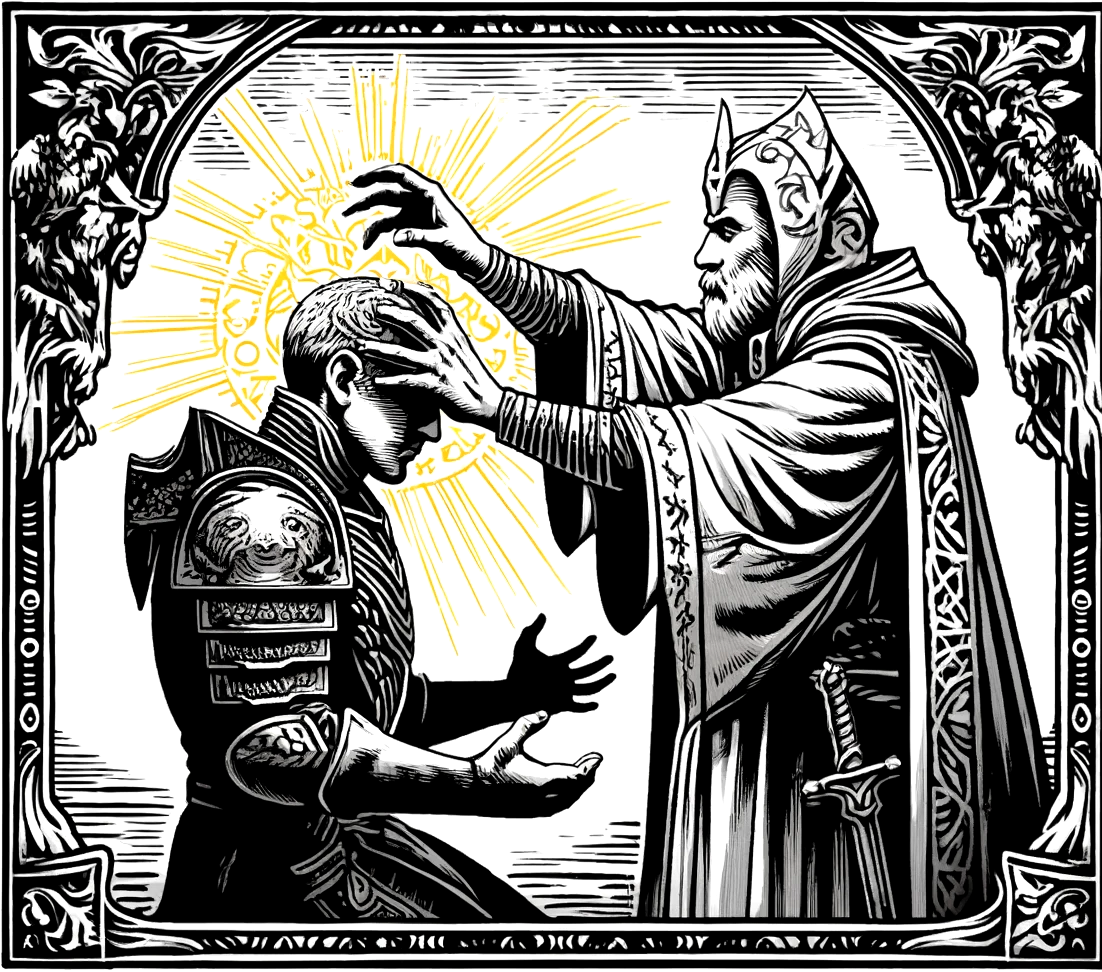
\includegraphics[width=0.7\textwidth]{spell_artwork/resistance.png}
\end{center}

\newpage
\section*{Sacred Flame}

{
\small\centering\vspace{-6pt}
\begin{tabular}{rlrl}
\toprule

\textbf{Duration:} & Instantaneous &
\textbf{Casting Time:} & 1 action \\
\textbf{Concentration:} & False &
\textbf{Range:} & 60 feet \\
\textbf{School:} & Evocation \\
\textbf{Components:} & \multicolumn{3}{p{0.7\textwidth}}{V, S}\\

\bottomrule
\end{tabular}
}

\vspace{1\baselineskip}\noindent 
\lettrine[lines=4]{
\includegraphics[height=58pt]{initials/F.png}}{lame-like radiance} descends on a creature that you can see within range. The target must succeed on a dexterity saving throw or take 1d8 radiant damage. The target gains no benefit from cover for this saving throw. The spell's damage increases by 1d8 when you reach 5th level (2d8), 11th level (3d8), and 17th level (4d8).

\newpage
\section*{Spare the Dying}

{
\small\centering\vspace{-6pt}
\begin{tabular}{rlrl}
\toprule

\textbf{Duration:} & Instantaneous &
\textbf{Casting Time:} & 1 action \\
\textbf{Concentration:} & False &
\textbf{Range:} & Touch \\
\textbf{School:} & Necromancy \\
\textbf{Components:} & \multicolumn{3}{p{0.7\textwidth}}{V, S}\\

\bottomrule
\end{tabular}
}

\vspace{1\baselineskip}\noindent 
\lettrine[lines=4]{
\includegraphics[height=58pt]{initials/Y.png}}{ou touch a} living creature that has 0 hit points. The creature becomes stable. This spell has no effect on undead or constructs.

\vfill
{
\centering

\includegraphics[width=0.85\textwidth]{spell_artwork/spare_the_dying.png}
}

\newpage
\section*{Thaumaturgy}

{
\small\centering\vspace{-6pt}
\begin{tabular}{rlrl}
\toprule

\textbf{Duration:} & 1 minute &
\textbf{Casting Time:} & 1 action \\
\textbf{Concentration:} & False &
\textbf{Range:} & 30 feet \\
\textbf{School:} & Transmutation \\
\textbf{Components:} & \multicolumn{3}{p{0.7\textwidth}}{V}\\

\bottomrule
\end{tabular}
}

\vspace{1\baselineskip}\noindent
\lettrine[lines=4]{
\includegraphics[height=58pt]{initials/Y.png}}{ou manifest a} minor wonder, a sign of supernatural power, within range. You create one of the following magical effects within range.
\vspace{6pt}
\begin{itemize}
    \item Your voice booms up to three times as loud as normal for 1 minute.
    \item You cause flames to flicker, brighten, dim, or change color for 1 minute.
    \item You cause harmless tremors in the ground for 1 minute.
    \item You create an instantaneous sound that originates from a point of your choice within range, such as a rumble of thunder, the cry of a raven, or ominous whispers.
    \item You instantaneously cause an unlocked door or window to fly open or slam shut.
    \item You alter the appearance of your eyes for 1 minute. If you cast this spell multiple times, you can have up to three of its 1-minute effects active at a time, and you can dismiss such an effect as an action.
\end{itemize}


\newpage
\begin{tikzpicture}[remember picture,overlay]
    \node[anchor=center] at (current page.center) {
        \includegraphics[height=1.1\pageheight]{spell_artwork/toll_of_the_dead.png}
    };
\end{tikzpicture}
\newpage
\section*{Toll the dead}
{
\small\centering\vspace{-6pt}
\begin{tabular}{rlrl}
\toprule

\textbf{Duration:} & Instantaneous  &
\textbf{Casting Time:} & 1 action \\
\textbf{Concentration:} & False &
\textbf{Range:} & 60 feet \\
\textbf{School:} & Necromancy \\
\textbf{Components:} & \multicolumn{3}{p{0.7\textwidth}}{V, S}\\

\bottomrule
\end{tabular}
}

\vspace{1\baselineskip}\noindent
\lettrine[lines=4]{
\includegraphics[height=58pt]{initials/Y.png}}{ou point at} one creature you can see within range, and the sound of a dolorous bell fills the air around it for a moment. The target must succeed on a Wisdom saving throw or take 1d8 necrotic damage. If the target is missing any of its hit points, it instead takes 1d12 necrotic damage.

\vspace{8pt} \noindent\textbf{At Higher Levels:} The spell’s damage increases by one die when you reach 5th level (2d8 or 2d12), 11th level (3d8 or 3d12), and 17th level (4d8 or 4d12).
\newpage
\section*{Word of Radiance}
{
\small\centering\vspace{-6pt}
\begin{tabular}{rlrl}
\toprule

\textbf{Duration:} & Instantaneous &
\textbf{Casting Time:} & 1 action \\
\textbf{Concentration:} & False &
\textbf{Range:} & 5 feet \\
\textbf{School:} & Evocation \\
\textbf{Components:} & \multicolumn{3}{p{0.7\textwidth}}{V, M (a holy symbol)}\\

\bottomrule
\end{tabular}
}

\vspace{1\baselineskip}\noindent
\lettrine[lines=4]{
\includegraphics[height=58pt]{initials/Y.png}}{ou utter a} divine word, and burning radiance erupts from you. Each creature of your choice that you can see within range must succeed on a Constitution saving throw or take 1d6 radiant damage.

\vspace{8pt} \noindent\textbf{At Higher Levels:} The spell’s damage increases by 1d6 when you reach 5th level (2d6), 11th level (3d6), and 17th level (4d6).
\newpage

\newpage
\chapter*{Level 1} \markboth{Level 1}{Level 1}

\section*{Bane}
\newpage

\section*{Bless}

{
\small\centering\vspace{-6pt}
\begin{tabular}{rlrl}
\toprule

\textbf{Duration:} & Up to 1 minute &
\textbf{Casting Time:} & 1 action \\
\textbf{Concentration:} & True &
\textbf{Range:} & 30 feet \\
\textbf{School:} & Enchantment \\
\textbf{Components:} & \multicolumn{3}{p{0.7\textwidth}}{V, S, M (A sprinkling of holy water.)}\\

\bottomrule
\end{tabular}
}

\vspace{1\baselineskip}\noindent
\lettrine[lines=4]{
\includegraphics[height=58pt]{initials/Y.png}}{ou bless up} to three creatures of your choice within range. Whenever a target makes an attack roll or a saving throw before the spell ends, the target can roll a d4 and add the number rolled to the attack roll or saving throw.

\vspace{8pt} \noindent\textbf{At Higher Levels:} When you cast this spell using a spell slot of 2nd level or higher, you can target one additional creature for each slot level above 1st.
\newpage
\section*{Command}

{
\small\centering\vspace{-6pt}
\begin{tabular}{rlrl}
\toprule

\textbf{Duration:} & 1 round &
\textbf{Casting Time:} & 1 action \\
\textbf{Concentration:} & False &
\textbf{Range:} & 60 feet \\
\textbf{School:} & Enchantment \\
\textbf{Components:} & \multicolumn{3}{p{0.7\textwidth}}{V}\\

\bottomrule
\end{tabular}
}

\vspace{1\baselineskip}\noindent 
\lettrine[lines=4]{
\includegraphics[height=58pt]{initials/Y.png}}{ou speak a} one-word command to a creature you can see within range. The target must succeed on a wisdom saving throw or follow the command on its next turn. The spell has no effect if the target is undead, if it doesn't understand your language, or if your command is directly harmful to it. Some typical commands and their effects follow. You might issue a command other than one described here. If you do so, the GM determines how the target behaves. If the target can't follow your command, the spell ends. \paragraph{Approach} The target moves toward you by the shortest and most direct route, ending its turn if it moves within 5 feet of you. \paragraph{Drop} The target drops whatever it is holding and then ends its turn. \paragraph{Flee} The target spends its turn moving away from you by the fastest available means. \paragraph{Grovel} The target falls prone and then ends its turn. \paragraph{Halt} The target doesn't move and takes no actions. A flying creature stays aloft, provided that it is able to do so. If it must move to stay aloft, it flies the minimum distance needed to remain in the air.

\vspace{8pt} \noindent\textbf{At Higher Levels:} When you cast this spell using a spell slot of 2nd level or higher, you can affect one additional creature for each slot level above 1st. The creatures must be within 30 feet of each other when you target them.
\newpage
\section*{Create or Destroy Water}

{
\small\centering\vspace{-6pt}
\begin{tabular}{rlrl}
\toprule

\textbf{Duration:} & Instantaneous &
\textbf{Casting Time:} & 1 action \\
\textbf{Concentration:} & False &
\textbf{Range:} & 30 feet \\
\textbf{School:} & Transmutation \\
\textbf{Components:} & \multicolumn{3}{p{0.7\textwidth}}{V, S, M (A drop of water if creating water, or a few grains of sand if destroying it.)}\\

\bottomrule
\end{tabular}
}

\vspace{1\baselineskip}\noindent
\lettrine[lines=4]{
\includegraphics[height=58pt]{initials/Y.png}}{ou either create} or destroy water.

\vspace{3\baselineskip}\noindent
\paragraph{Create Water} You create up to 10 gallons of clean water within range in an open container. Alternatively, the water falls as rain in a 30-foot cube within range. \paragraph{Destroy Water} You destroy up to 10 gallons of water in an open container within range. Alternatively, you destroy fog in a 30-foot cube within range.

\vspace{8pt} \noindent\textbf{At Higher Levels:} When you cast this spell using a spell slot of 2nd level or higher, you create or destroy 10 additional gallons of water, or the size of the cube increases by 5 feet, for each slot level above 1st.
\newpage
\begin{tikzpicture}[remember picture,overlay]
    \node[anchor=center] at (current page.center) {
        \includegraphics[height=1.1\pageheight]{spell_artwork/cure_wounds.png}
    };
\end{tikzpicture}
\newpage
\section*{Cure Wounds}
\newpage
\section*{Detect Evil and Good}

{
\small\centering\vspace{-6pt}
\begin{tabular}{rlrl}
\toprule

\textbf{Duration:} & Up to 10 minutes &
\textbf{Casting Time:} & 1 action \\
\textbf{Concentration:} & True &
\textbf{Range:} & Self \\
\textbf{School:} & Divination \\
\textbf{Components:} & \multicolumn{3}{p{0.7\textwidth}}{V, S}\\

\bottomrule
\end{tabular}
}

\vspace{1\baselineskip}\noindent
\lettrine[lines=4]{
\includegraphics[height=58pt]{initials/F.png}}{or the duration}, you know if there is an aberration, celestial, elemental, fey, fiend, or undead within 30 feet of you, as well as where the creature is located. Similarly, you know if there is a place or object within 30 feet of you that has been magically consecrated or desecrated. The spell can penetrate most barriers, but it is blocked by 1 foot of stone, 1 inch of common metal, a thin sheet of lead, or 3 feet of wood or dirt.

\newpage
\section*{Detect Magic}
\newpage
\section*{Detect Poison and Disease}

{
\small\centering\vspace{-6pt}
\begin{tabular}{rlrl}
\toprule

\textbf{Duration:} & Up to 10 minutes &
\textbf{Casting Time:} & 1 action \\
\textbf{Concentration:} & True &
\textbf{Range:} & Self \\
\textbf{School:} & Divination \\
\textbf{Components:} & \multicolumn{3}{p{0.7\textwidth}}{V, S, M (A yew leaf.)}\\

\bottomrule
\end{tabular}
}

\vspace{1\baselineskip}\noindent
\lettrine[lines=4]{
\includegraphics[height=58pt]{initials/F.png}}{or the duration}, you can sense the presence and location of poisons, poisonous creatures, and diseases within 30 feet of you. You also identify the kind of poison, poisonous creature, or disease in each case. The spell can penetrate most barriers, but it is blocked by 1 foot of stone, 1 inch of common metal, a thin sheet of lead, or 3 feet of wood or dirt.

\newpage
\section*{Guiding Bolt}

{
\small\centering\vspace{-6pt}
\begin{tabular}{rlrl}
\toprule

\textbf{Duration:} & 1 round &
\textbf{Casting Time:} & 1 action \\
\textbf{Concentration:} & False &
\textbf{Range:} & 120 feet \\
\textbf{School:} & Evocation \\
\textbf{Components:} & \multicolumn{3}{p{0.7\textwidth}}{V, S}\\

\bottomrule
\end{tabular}
}

\vspace{1\baselineskip}\noindent
\lettrine[lines=4]{
\includegraphics[height=66pt]{initials/A.png}}{\ flash of light} streaks toward a creature of your choice within range. Make a ranged spell attack against the target. On a hit, the target takes 4d6 radiant damage, and the next attack roll made against this target before the end of your next turn has advantage, thanks to the mystical dim light glittering on the target until then.

\vspace{8pt} \noindent\textbf{At Higher Levels:} When you cast this spell using a spell slot of 2nd level or higher, the damage increases by 1d6 for each slot level above 1st.
\newpage
\begin{tikzpicture}[remember picture,overlay]
    \node[anchor=center] at (current page.center) {
        \includegraphics[height=1.1\pageheight]{spell_artwork/healing_word.png}
    };
\end{tikzpicture}
\newpage
\section*{Healing Word}
\newpage
\section*{Inflict Wounds}

{
\small\centering\vspace{-6pt}
\begin{tabular}{rlrl}
\toprule

\textbf{Duration:} & Instantaneous &
\textbf{Casting Time:} & 1 action \\
\textbf{Concentration:} & False &
\textbf{Range:} & Touch \\
\textbf{School:} & Necromancy \\
\textbf{Components:} & \multicolumn{3}{p{0.7\textwidth}}{V, S}\\

\bottomrule
\end{tabular}
}

\vspace{1\baselineskip}\noindent
\lettrine[lines=4]{
\includegraphics[height=56pt]{initials/M.png}}{ake a melee} spell attack against a creature you can reach. On a hit, the target takes 3d10 necrotic damage.

\vspace{2\baselineskip}\noindent
\textbf{At Higher Levels:} When you cast this spell using a spell slot of 2nd level or higher, the damage increases by 1d10 for each slot level above 1st.
\newpage
\section*{Protection from Evil and Good}

{
\small\centering\vspace{-6pt}
\begin{tabular}{rlrl}
\toprule

\textbf{Duration:} & Up to 10 minutes &
\textbf{Casting Time:} & 1 action \\
\textbf{Concentration:} & True &
\textbf{Range:} & Touch \\
\textbf{School:} & Abjuration \\
\textbf{Components:} & \multicolumn{3}{p{0.7\textwidth}}{V, S, M (Holy water or powdered silver and iron, which the spell consumes.)}\\

\bottomrule
\end{tabular}
}

\vspace{1\baselineskip}\noindent 
\lettrine[lines=4]{
\includegraphics[height=60pt]{initials/U.png}}{ntil the spell} ends, one willing creature you touch is protected against certain types of creatures: aberrations, celestials, elementals, fey, fiends, and undead. The protection grants several benefits. Creatures of those types have disadvantage on attack rolls against the target. The target also can't be charmed, frightened, or possessed by them. If the target is already charmed, frightened, or possessed by such a creature, the target has advantage on any new saving throw against the relevant effect.

\newpage
\section*{Purify Food and Drink}

{
\small\centering\vspace{-6pt}
\begin{tabular}{rlrl}
\toprule

\textbf{Duration:} & Instantaneous &
\textbf{Casting Time:} & 1 action \\
\textbf{Concentration:} & False &
\textbf{Range:} & 10 feet \\
\textbf{School:} & Transmutation \\
\textbf{Components:} & \multicolumn{3}{p{0.7\textwidth}}{V, S}\\

\bottomrule
\end{tabular}
}

\vspace{1\baselineskip}\noindent 
\lettrine[lines=4]{
\includegraphics[height=66pt]{initials/A.png}}{ll nonmagical food} and drink within a 5-foot radius sphere centered on a point of your choice within range is purified and rendered free of poison and disease.

\newpage
\section*{Sanctuary}

{
\small\centering\vspace{-6pt}
\begin{tabular}{rlrl}
\toprule

\textbf{Duration:} & 1 minute &
\textbf{Casting Time:} & 1 bonus action \\
\textbf{Concentration:} & False &
\textbf{Range:} & 30 feet \\
\textbf{School:} & Abjuration \\
\textbf{Components:} & \multicolumn{3}{p{0.7\textwidth}}{V, S, M (A small silver mirror.)}\\

\bottomrule
\end{tabular}
}

\vspace{1\baselineskip}\noindent
\lettrine[lines=4]{
\includegraphics[height=58pt]{initials/Y.png}}{ou ward a} creature within range against attack. Until the spell ends, any creature who targets the warded creature with an attack or a harmful spell must first make a wisdom saving throw. On a failed save, the creature must choose a new target or lose the attack or spell. This spell doesn't protect the warded creature from area effects, such as the explosion of a fireball. If the warded creature makes an attack or casts a spell that affects an enemy creature, this spell ends.

\newpage
\section*{Shield of Faith}

{
\small\centering\vspace{-6pt}
\begin{tabular}{rlrl}
\toprule

\textbf{Duration:} & Up to 10 minutes &
\textbf{Casting Time:} & 1 bonus action \\
\textbf{Concentration:} & True &
\textbf{Range:} & 60 feet \\
\textbf{School:} & Abjuration \\
\textbf{Components:} & \multicolumn{3}{p{0.7\textwidth}}{V, S, M (A small parchment with a bit of holy text written on it.)}\\

\bottomrule
\end{tabular}
}

\vspace{1\baselineskip}\noindent A shimmering field appears and surrounds a creature of your choice within range, granting it a +2 bonus to AC for the duration.

\newpage
\chapter*{Level 2} \markboth{Level 2}{Level 2}
\section*{Aid}

{
\small\centering\vspace{-6pt}
\begin{tabular}{rlrl}
\toprule

\textbf{Duration:} & 8 hours &
\textbf{Casting Time:} & 1 action \\
\textbf{Concentration:} & False &
\textbf{Range:} & 30 feet \\
\textbf{School:} & Abjuration \\
\textbf{Components:} & \multicolumn{3}{p{0.7\textwidth}}{V, S, M (A tiny strip of white cloth.)}\\

\bottomrule
\end{tabular}
}

\vspace{1\baselineskip}\noindent 
\lettrine[lines=4]{
\includegraphics[height=58pt]{initials/Y.png}}{our spell bolsters} your allies with toughness and resolve. Choose up to three creatures within range. Each target's hit point maximum and current hit points increase by 5 for the duration.

\vspace{8pt} \noindent\textbf{At Higher Levels:} When you cast this spell using a spell slot of 3rd level or higher, a target's hit points increase by an additional 5 for each slot level above 2nd.
\newpage
\section*{Augury}

{
\small\centering\vspace{-6pt}
\begin{tabular}{rlrl}
\toprule

\textbf{Duration:} & Instantaneous &
\textbf{Casting Time:} & 1 minute \\
\textbf{Concentration:} & False &
\textbf{Range:} & Self \\
\textbf{School:} & Divination \\
\textbf{Components:} & \multicolumn{3}{p{0.7\textwidth}}{V, S, M (Specially marked sticks, bones, or similar tokens worth at least 25gp.)}\\

\bottomrule
\end{tabular}
}

\vspace{1\baselineskip}\noindent By casting gem-inlaid sticks, rolling dragon bones, laying out ornate cards, or employing some other divining tool, you receive an omen from an otherworldly entity about the results of a specific course of action that you plan to take within the next 30 minutes. The GM chooses from the following possible omens:
\begin{itemize}
    \item Weal, for good results
    \item Woe, for bad results
    \item Weal and woe, for both good and bad results
    \item Nothing, for results that aren't especially good or bad The spell doesn't take into account any possible circumstances that might change the outcome, such as the casting of additional spells or the loss or gain of a companion. If you cast the spell two or more times before completing your next long rest, there is a cumulative 25 percent chance for each casting after the first that you get a random reading. The GM makes this roll in secret.
\end{itemize}


\newpage
\section*{Continual Flame}

{
\small\centering\vspace{-6pt}
\begin{tabular}{rlrl}
\toprule

\textbf{Duration:} & Until dispelled &
\textbf{Casting Time:} & 1 action \\
\textbf{Concentration:} & False &
\textbf{Range:} & Touch \\
\textbf{School:} & Evocation \\
\textbf{Components:} & \multicolumn{3}{p{0.7\textwidth}}{V, S, M (Ruby dust worth 50 gp, which the spell consumes.)}\\

\bottomrule
\end{tabular}
}

\vspace{1\baselineskip}\noindent A flame, equivalent in brightness to a torch, springs forth from an object that you touch. The effect looks like a regular flame, but it creates no heat and doesn't use oxygen. A continual flame can be covered or hidden but not smothered or quenched.

\newpage
\section*{Find Traps}

{
\small\centering\vspace{-6pt}
\begin{tabular}{rlrl}
\toprule

\textbf{Duration:} & Instantaneous &
\textbf{Casting Time:} & 1 action \\
\textbf{Concentration:} & False &
\textbf{Range:} & 120 feet \\
\textbf{School:} & Divination \\
\textbf{Components:} & \multicolumn{3}{p{0.7\textwidth}}{V, S}\\

\bottomrule
\end{tabular}
}

\vspace{1\baselineskip}\noindent
\lettrine[lines=4]{
\includegraphics[height=58pt]{initials/Y.png}}{ou sense the} presence of any trap within range that is within line of sight. A trap, for the purpose of this spell, includes anything that would inflict a sudden or unexpected effect you consider harmful or undesirable, which was specifically intended as such by its creator. Thus, the spell would sense an area affected by the alarm spell, a glyph of warding, or a mechanical pit trap, but it would not reveal a natural weakness in the floor, an unstable ceiling, or a hidden sinkhole. This spell merely reveals that a trap is present. You don't learn the location of each trap, but you do learn the general nature of the danger posed by a trap you sense.

\newpage
\section*{Gentle Repose}

{
\small\centering\vspace{-6pt}
\begin{tabular}{rlrl}
\toprule

\textbf{Duration:} & 10 days &
\textbf{Casting Time:} & 1 action \\
\textbf{Concentration:} & False &
\textbf{Range:} & Touch \\
\textbf{School:} & Necromancy \\
\textbf{Components:} & \multicolumn{3}{p{0.7\textwidth}}{V, S, M (A pinch of salt and one copper piece placed on each of the corpse's eyes, which must remain there for the duration.)}\\

\bottomrule
\end{tabular}
}

\vspace{1\baselineskip}\noindent 
\lettrine[lines=4]{
\includegraphics[height=58pt]{initials/Y.png}}{ou touch a} corpse or other remains. For the duration, the target is protected from decay and can't become undead. The spell also effectively extends the time limit on raising the target from the dead, since days spent under the influence of this spell don't count against the time limit of spells such as raise dead.

\newpage
\section*{Prayer of Healing}

{
\small\centering\vspace{-6pt}
\begin{tabular}{rlrl}
\toprule

\textbf{Duration:} & Instantaneous &
\textbf{Casting Time:} & 10 minutes \\
\textbf{Concentration:} & False &
\textbf{Range:} & 30 feet \\
\textbf{School:} & Evocation \\
\textbf{Components:} & \multicolumn{3}{p{0.7\textwidth}}{V}\\

\bottomrule
\end{tabular}
}

\vspace{1\baselineskip}\noindent Up to six creatures of your choice that you can see within range each regain hit points equal to 2d8 + your spellcasting ability modifier. This spell has no effect on undead or constructs.

\vspace{8pt} \noindent\textbf{At Higher Levels:} When you cast this spell using a spell slot of 3rd level or higher, the healing increases by 1d8 for each slot level above 2nd.
\newpage
\section*{Protection from Poison}

{
\small\centering\vspace{-6pt}
\begin{tabular}{rlrl}
\toprule

\textbf{Duration:} & 1 hour &
\textbf{Casting Time:} & 1 action \\
\textbf{Concentration:} & False &
\textbf{Range:} & Touch \\
\textbf{School:} & Abjuration \\
\textbf{Components:} & \multicolumn{3}{p{0.7\textwidth}}{V, S}\\

\bottomrule
\end{tabular}
}

\vspace{1\baselineskip}\noindent 
\lettrine[lines=4]{
\includegraphics[height=58pt]{initials/Y.png}}{ou touch a} creature. If it is poisoned, you neutralize the poison. If more than one poison afflicts the target, you neutralize one poison that you know is present, or you neutralize one at random. For the duration, the target has advantage on saving throws against being poisoned, and it has resistance to poison damage.

\newpage
\section*{Spiritual Weapon}

{
\small\centering\vspace{-6pt}
\begin{tabular}{rlrl}
\toprule

\textbf{Duration:} & 1 minute &
\textbf{Casting Time:} & 1 bonus action \\
\textbf{Concentration:} & False &
\textbf{Range:} & 60 feet \\
\textbf{School:} & Evocation \\
\textbf{Components:} & \multicolumn{3}{p{0.7\textwidth}}{V, S}\\

\bottomrule
\end{tabular}
}

\vspace{1\baselineskip}\noindent 
\lettrine[lines=4]{
\includegraphics[height=58pt]{initials/Y.png}}{ou create a} floating, spectral weapon within range that lasts for the duration or until you cast this spell again. When you cast the spell, you can make a melee spell attack against a creature within 5 feet of the weapon. On a hit, the target takes force damage equal to 1d8 + your spellcasting ability modifier. As a bonus action on your turn, you can move the weapon up to 20 feet and repeat the attack against a creature within 5 feet of it. The weapon can take whatever form you choose. Clerics of deities who are associated with a particular weapon (as St. Cuthbert is known for his mace and Thor for his hammer) make this spell's effect resemble that weapon.

\vspace{8pt} \noindent\textbf{At Higher Levels:} When you cast this spell using a spell slot of 3rd level or higher, the damage increases by 1d8 for every two slot levels above the 2nd.
\newpage
\section*{Warding Bond}

{
\small\centering\vspace{-6pt}
\begin{tabular}{rlrl}
\toprule

\textbf{Duration:} & 1 hour &
\textbf{Casting Time:} & 1 action \\
\textbf{Concentration:} & False &
\textbf{Range:} & Touch \\
\textbf{School:} & Abjuration \\
\textbf{Components:} & \multicolumn{3}{p{0.7\textwidth}}{V, S, M (A pair of platinum rings worth at least 50gp each, which you and the target must wear for the duration.)}\\

\bottomrule
\end{tabular}
}

\vspace{1\baselineskip}\noindent This spell wards a willing creature you touch and creates a mystic connection between you and the target until the spell ends. While the target is within 60 feet of you, it gains a +1 bonus to AC and saving throws, and it has resistance to all damage. Also, each time it takes damage, you take the same amount of damage. The spell ends if you drop to 0 hit points or if you and the target become separated by more than 60 feet. It also ends if the spell is cast again on either of the connected creatures. You can also dismiss the spell as an action.

\newpage
\chapter*{Level 3} \markboth{Level 3}{Level 3}
\section*{Animate Dead}

{
\small\centering\vspace{-6pt}
\begin{tabular}{rlrl}
\toprule

\textbf{Duration:} & Instantaneous &
\textbf{Casting Time:} & 1 minute \\
\textbf{Concentration:} & False &
\textbf{Range:} & 10 feet \\
\textbf{School:} & Necromancy \\
\textbf{Components:} & \multicolumn{3}{p{0.7\textwidth}}{V, S, M (A drop of blood, a piece of flesh, and a pinch of bone dust.)}\\

\bottomrule
\end{tabular}
}

\vspace{1\baselineskip}\noindent This spell creates an undead servant. Choose a pile of bones or a corpse of a Medium or Small humanoid within range. Your spell imbues the target with a foul mimicry of life, raising it as an undead creature. The target becomes a skeleton if you chose bones or a zombie if you chose a corpse (the GM has the creature's game statistics). On each of your turns, you can use a bonus action to mentally command any creature you made with this spell if the creature is within 60 feet of you (if you control multiple creatures, you can command any or all of them at the same time, issuing the same command to each one). You decide what action the creature will take and where it will move during its next turn, or you can issue a general command, such as to guard a particular chamber or corridor. If you issue no commands, the creature only defends itself against hostile creatures. Once given an order, the creature continues to follow it until its task is complete. The creature is under your control for 24 hours, after which it stops obeying any command you've given it. To maintain control of the creature for another 24 hours, you must cast this spell on the creature again before the current 24-hour period ends. This use of the spell reasserts your control over up to four creatures you have animated with this spell, rather than animating a new one.

\vspace{8pt} \noindent\textbf{At Higher Levels:} When you cast this spell using a spell slot of 4th level or higher, you animate or reassert control over two additional undead creatures for each slot level above 3rd. Each of the creatures must come from a different corpse or pile of bones.
\newpage
\section*{Beacon of Hope}

{
\small\centering\vspace{-6pt}
\begin{tabular}{rlrl}
\toprule

\textbf{Duration:} & Up to 1 minute &
\textbf{Casting Time:} & 1 action \\
\textbf{Concentration:} & True &
\textbf{Range:} & 30 feet \\
\textbf{School:} & Abjuration \\
\textbf{Components:} & \multicolumn{3}{p{0.7\textwidth}}{V, S}\\

\bottomrule
\end{tabular}
}

\vspace{1\baselineskip}\noindent This spell bestows hope and vitality. Choose any number of creatures within range. For the duration, each target has advantage on wisdom saving throws and death saving throws, and regains the maximum number of hit points possible from any healing.

\newpage
\section*{Create Food and Water}

{
\small\centering\vspace{-6pt}
\begin{tabular}{rlrl}
\toprule

\textbf{Duration:} & Instantaneous &
\textbf{Casting Time:} & 1 action \\
\textbf{Concentration:} & False &
\textbf{Range:} & 30 feet \\
\textbf{School:} & Conjuration \\
\textbf{Components:} & \multicolumn{3}{p{0.7\textwidth}}{V, S}\\

\bottomrule
\end{tabular}
}

\vspace{1\baselineskip}\noindent 
\lettrine[lines=4]{
\includegraphics[height=58pt]{initials/Y.png}}{ou create 45} pounds of food and 30 gallons of water on the ground or in containers within range, enough to sustain up to fifteen humanoids or five steeds for 24 hours. The food is bland but nourishing, and spoils if uneaten after 24 hours. The water is clean and doesn't go bad.

\newpage
\section*{Daylight}

{
\small\centering\vspace{-6pt}
\begin{tabular}{rlrl}
\toprule

\textbf{Duration:} & 1 hour &
\textbf{Casting Time:} & 1 action \\
\textbf{Concentration:} & False &
\textbf{Range:} & 60 feet \\
\textbf{School:} & Evocation \\
\textbf{Components:} & \multicolumn{3}{p{0.7\textwidth}}{V, S}\\

\bottomrule
\end{tabular}
}

\vspace{1\baselineskip}\noindent A 60-foot-radius sphere of light spreads out from a point you choose within range. The sphere is bright light and sheds dim light for an additional 60 feet. If you chose a point on an object you are holding or one that isn't being worn or carried, the light shines from the object and moves with it. Completely covering the affected object with an opaque object, such as a bowl or a helm, blocks the light. If any of this spell's area overlaps with an area of darkness created by a spell of 3rd level or lower, the spell that created the darkness is dispelled.

\newpage
\section*{Magic Circle}

{
\small\centering\vspace{-6pt}
\begin{tabular}{rlrl}
\toprule

\textbf{Duration:} & 1 hour &
\textbf{Casting Time:} & 1 minute \\
\textbf{Concentration:} & False &
\textbf{Range:} & 10 feet \\
\textbf{School:} & Abjuration \\
\textbf{Components:} & \multicolumn{3}{p{0.7\textwidth}}{V, S, M (Holy water or powdered silver and iron worth at least 100 gp, which the spell consumes.)}\\

\bottomrule
\end{tabular}
}

\vspace{1\baselineskip}\noindent
\lettrine[lines=4]{
\includegraphics[height=58pt]{initials/Y.png}}{ou create a} 10-foot radius, 20-foot-tall cylinder of magical energy centered on a point on the ground that you can see within range. Glowing runes appear whenever the cylinder intersects with the floor or other surface. Choose one or more of the following types of creatures: celestials, elementals, fey, fiends, or undead. The circle affects a creature of the chosen type in the following ways:
\begin{itemize}
    \item The creature can't willingly enter the cylinder by nonmagical means. If the creature tries to use teleportation or interplanar travel to do so, it must first succeed on a charisma saving throw.
    \item The creature has disadvantage on attack rolls against targets within the cylinder.
    \item Targets within the cylinder can't be charmed, frightened, or possessed by the creature. When you cast this spell, you can elect to cause its magic to operate in the reverse direction, preventing a creature of the specified type from leaving the cylinder and protecting targets outside it.
\end{itemize}


\vspace{8pt} \noindent\textbf{At Higher Levels:} When you cast this spell using a spell slot of 4th level or higher, the duration increases by 1 hour for each slot level above 3rd.
\newpage
\section*{Mass Healing Word}

{
\small\centering\vspace{-6pt}
\begin{tabular}{rlrl}
\toprule

\textbf{Duration:} & Instantaneous &
\textbf{Casting Time:} & 1 bonus action \\
\textbf{Concentration:} & False &
\textbf{Range:} & 60 feet \\
\textbf{School:} & Evocation \\
\textbf{Components:} & \multicolumn{3}{p{0.7\textwidth}}{V}\\

\bottomrule
\end{tabular}
}

\vspace{1\baselineskip}\noindent As you call out words of restoration, up to six creatures of your choice that you can see within range regain hit points equal to 1d4 + your spellcasting ability modifier. This spell has no effect on undead or constructs.

\vspace{8pt} \noindent\textbf{At Higher Levels:} When you cast this spell using a spell slot of 4th level or higher, the healing increases by 1d4 for each slot level above 3rd.
\newpage
\section*{Meld Into Stone}

{
\small\centering\vspace{-6pt}
\begin{tabular}{rlrl}
\toprule

\textbf{Duration:} & 8 hours &
\textbf{Casting Time:} & 1 action \\
\textbf{Concentration:} & False &
\textbf{Range:} & Touch \\
\textbf{School:} & Transmutation \\
\textbf{Components:} & \multicolumn{3}{p{0.7\textwidth}}{V, S}\\

\bottomrule
\end{tabular}
}

\vspace{1\baselineskip}\noindent 
\lettrine[lines=4]{
\includegraphics[height=58pt]{initials/Y.png}}{ou step into} a stone object or surface large enough to fully contain your body, melding yourself and all the equipment you carry with the stone for the duration. Using your movement, you step into the stone at a point you can touch. Nothing of your presence remains visible or otherwise detectable by nonmagical senses. While merged with the stone, you can't see what occurs outside it, and any Wisdom (Perception) checks you make to hear sounds outside it are made with disadvantage. You remain aware of the passage of time and can cast spells on yourself while merged in the stone. You can use your movement to leave the stone where you entered it, which ends the spell. You otherwise can't move. Minor physical damage to the stone doesn't harm you, but its partial destruction or a change in its shape (to the extent that you no longer fit within it) expels you and deals 6d6 bludgeoning damage to you. The stone's complete destruction (or transmutation into a different substance) expels you and deals 50 bludgeoning damage to you. If expelled, you fall prone in an unoccupied space closest to where you first entered.

\newpage
\section*{Protection From Energy}

{
\small\centering\vspace{-6pt}
\begin{tabular}{rlrl}
\toprule

\textbf{Duration:} & Up to 1 hour &
\textbf{Casting Time:} & 1 action \\
\textbf{Concentration:} & True &
\textbf{Range:} & Touch \\
\textbf{School:} & Abjuration \\
\textbf{Components:} & \multicolumn{3}{p{0.7\textwidth}}{V, S}\\

\bottomrule
\end{tabular}
}

\vspace{1\baselineskip}\noindent For the duration, the willing creature you touch has resistance to one damage type of your choice: acid, cold, fire, lightning, or thunder.

\newpage
\section*{Remove Curse}

{
\small\centering\vspace{-6pt}
\begin{tabular}{rlrl}
\toprule

\textbf{Duration:} & Instantaneous &
\textbf{Casting Time:} & 1 action \\
\textbf{Concentration:} & False &
\textbf{Range:} & Touch \\
\textbf{School:} & Abjuration \\
\textbf{Components:} & \multicolumn{3}{p{0.7\textwidth}}{V, S}\\

\bottomrule
\end{tabular}
}

\vspace{1\baselineskip}\noindent At your touch, all curses affecting one creature or object end. If the object is a cursed magic item, its curse remains, but the spell breaks its owner's attunement to the object so it can be removed or discarded.

\newpage
\section*{Revivify}

{
\small\centering\vspace{-6pt}
\begin{tabular}{rlrl}
\toprule

\textbf{Duration:} & Instantaneous &
\textbf{Casting Time:} & 1 action \\
\textbf{Concentration:} & False &
\textbf{Range:} & Touch \\
\textbf{School:} & Conjuration \\
\textbf{Components:} & \multicolumn{3}{p{0.7\textwidth}}{V, S, M (Diamonds worth 300gp, which the spell consumes.)}\\

\bottomrule
\end{tabular}
}

\vspace{1\baselineskip}\noindent 
\lettrine[lines=4]{
\includegraphics[height=58pt]{initials/Y.png}}{ou touch a} creature that has died within the last minute. That creature returns to life with 1 hit point. This spell can't return to life a creature that has died of old age, nor can it restore any missing body parts.

\newpage
\section*{Spirit Guardians}

{
\small\centering\vspace{-6pt}
\begin{tabular}{rlrl}
\toprule

\textbf{Duration:} & Up to 10 minutes &
\textbf{Casting Time:} & 1 action \\
\textbf{Concentration:} & True &
\textbf{Range:} & Self \\
\textbf{School:} & Conjuration \\
\textbf{Components:} & \multicolumn{3}{p{0.7\textwidth}}{V, S, M (A holy symbol.)}\\

\bottomrule
\end{tabular}
}

\vspace{1\baselineskip}\noindent 
\lettrine[lines=4]{
\includegraphics[height=58pt]{initials/Y.png}}{ou call forth} spirits to protect you. They flit around you to a distance of 15 feet for the duration. If you are good or neutral, their spectral form appears angelic or fey (your choice). If you are evil, they appear fiendish. When you cast this spell, you can designate any number of creatures you can see to be unaffected by it. An affected creature's speed is halved in the area, and when the creature enters the area for the first time on a turn or starts its turn there, it must make a wisdom saving throw. On a failed save, the creature takes 3d8 radiant damage (if you are good or neutral) or 3d8 necrotic damage (if you are evil). On a successful save, the creature takes half as much damage.

\vspace{8pt} \noindent\textbf{At Higher Levels:} When you cast this spell using a spell slot of 4th level or higher, the damage increases by 1d8 for each slot level above 3rd.
\newpage
\section*{Water Walk}

{
\small\centering\vspace{-6pt}
\begin{tabular}{rlrl}
\toprule

\textbf{Duration:} & 1 hour &
\textbf{Casting Time:} & 1 action \\
\textbf{Concentration:} & False &
\textbf{Range:} & 30 feet \\
\textbf{School:} & Transmutation \\
\textbf{Components:} & \multicolumn{3}{p{0.7\textwidth}}{V, S, M (A piece of cork.)}\\

\bottomrule
\end{tabular}
}

\vspace{1\baselineskip}\noindent This spell grants the ability to move across any liquid surface--such as water, acid, mud, snow, quicksand, or lava--as if it were harmless solid ground (creatures crossing molten lava can still take damage from the heat). Up to ten willing creatures you can see within range gain this ability for the duration. If you target a creature submerged in a liquid, the spell carries the target to the surface of the liquid at a rate of 60 feet per round.

\newpage
\chapter*{Level 4} \markboth{Level 4}{Level 4}
\section*{Arcane Eye}

{
\small\centering\vspace{-6pt}
\begin{tabular}{rlrl}
\toprule

\textbf{Duration:} & Up to 1 hour &
\textbf{Casting Time:} & 1 action \\
\textbf{Concentration:} & True &
\textbf{Range:} & 30 feet \\
\textbf{School:} & Divination \\
\textbf{Components:} & \multicolumn{3}{p{0.7\textwidth}}{V, S, M (A bit of bat fur.)}\\

\bottomrule
\end{tabular}
}

\vspace{1\baselineskip}\noindent 
\lettrine[lines=4]{
\includegraphics[height=58pt]{initials/Y.png}}{ou create an} invisible, magical eye within range that hovers in the air for the duration. You mentally receive visual information from the eye, which has normal vision and darkvision out to 30 feet. The eye can look in every direction. As an action, you can move the eye up to 30 feet in any direction. There is no limit to how far away from you the eye can move, but it can't enter another plane of existence. A solid barrier blocks the eye's movement, but the eye can pass through an opening as small as 1 inch in diameter.

\newpage
\section*{Banishment}

{
\small\centering\vspace{-6pt}
\begin{tabular}{rlrl}
\toprule

\textbf{Duration:} & Up to 1 minute &
\textbf{Casting Time:} & 1 action \\
\textbf{Concentration:} & True &
\textbf{Range:} & 60 feet \\
\textbf{School:} & Abjuration \\
\textbf{Components:} & \multicolumn{3}{p{0.7\textwidth}}{V, S, M (An item distasteful to the target.)}\\

\bottomrule
\end{tabular}
}

\vspace{1\baselineskip}\noindent 
\lettrine[lines=4]{
\includegraphics[height=58pt]{initials/Y.png}}{ou attempt to} send one creature that you can see within range to another plane of existence. The target must succeed on a charisma saving throw or be banished. If the target is native to the plane of existence you're on, you banish the target to a harmless demiplane. While there, the target is incapacitated. The target remains there until the spell ends, at which point the target reappears in the space it left or in the nearest unoccupied space if that space is occupied. If the target is native to a different plane of existence than the one you're on, the target is banished with a faint popping noise, returning to its home plane. If the spell ends before 1 minute has passed, the target reappears in the space it left or in the nearest unoccupied space if that space is occupied. Otherwise, the target doesn't return.

\vspace{8pt} \noindent\textbf{At Higher Levels:} When you cast this spell using a spell slot of 5th level or higher, you can target one additional creature for each slot level above 4th.
\newpage
\section*{Control Water}

{
\small\centering\vspace{-6pt}
\begin{tabular}{rlrl}
\toprule

\textbf{Duration:} & Up to 10 minutes &
\textbf{Casting Time:} & 1 action \\
\textbf{Concentration:} & True &
\textbf{Range:} & 300 feet \\
\textbf{School:} & Transmutation \\
\textbf{Components:} & \multicolumn{3}{p{0.7\textwidth}}{V, S, M (A drop of water and a pinch of dust.)}\\

\bottomrule
\end{tabular}
}

\vspace{1\baselineskip}\noindent Until the spell ends, you control any freestanding water inside an area you choose that is a cube up to 100 feet on a side. You can choose from any of the following effects when you cast this spell. As an action on your turn, you can repeat the same effect or choose a different one. \paragraph{Flood} You cause the water level of all standing water in the area to rise by as much as 20 feet. If the area includes a shore, the flooding water spills over onto dry land. If you choose an area in a large body of water, you instead create a 20-foot tall wave that travels from one side of the area to the other and then crashes down. Any Huge or smaller vehicles in the wave's path are carried with it to the other side. Any Huge or smaller vehicles struck by the wave have a 25 percent chance of capsizing. The water level remains elevated until the spell ends or you choose a different effect. If this effect produced a wave, the wave repeats on the start of your next turn while the flood effect lasts. \paragraph{Part Water} You cause water in the area to move apart and create a trench. The trench extends across the spell's area, and the separated water forms a wall to either side. The trench remains until the spell ends or you choose a different effect. The water then slowly fills in the trench over the course of the next round until the normal water level is restored. \paragraph{Redirect Flow} You cause flowing water in the area to move in a direction you choose, even if the water has to flow over obstacles, up walls, or in other unlikely directions. The water in the area moves as you direct it, but once it moves beyond the spell's area, it resumes its flow based on the terrain conditions. The water continues to move in the direction you chose until the spell ends or you choose a different effect. \paragraph{Whirlpool} This effect requires a body of water at least 50 feet square and 25 feet deep. You cause a whirlpool to form in the center of the area. The whirlpool forms a vortex that is 5 feet wide at the base, up to 50 feet wide at the top, and 25 feet tall. Any creature or object in the water and within 25 feet of the vortex is pulled 10 feet toward it. A creature can swim away from the vortex by making a Strength (Athletics) check against your spell save DC. When a creature enters the vortex for the first time on a turn or starts its turn there, it must make a strength saving throw. On a failed save, the creature takes 2d8 bludgeoning damage and is caught in the vortex until the spell ends. On a successful save, the creature takes half damage, and isn't caught in the vortex. A creature caught in the vortex can use its action to try to swim away from the vortex as described above, but has disadvantage on the Strength (Athletics) check to do so. The first time each turn that an object enters the vortex, the object takes 2d8 bludgeoning damage; this damage occurs each round it remains in the vortex.

\newpage
\section*{Death Ward}

{
\small\centering\vspace{-6pt}
\begin{tabular}{rlrl}
\toprule

\textbf{Duration:} & 8 hours &
\textbf{Casting Time:} & 1 action \\
\textbf{Concentration:} & False &
\textbf{Range:} & Touch \\
\textbf{School:} & Abjuration \\
\textbf{Components:} & \multicolumn{3}{p{0.7\textwidth}}{V, S}\\

\bottomrule
\end{tabular}
}

\vspace{1\baselineskip}\noindent You touch a creature and grant it a measure of protection from death. The first time the target would drop to 0 hit points as a result of taking damage, the target instead drops to 1 hit point, and the spell ends. If the spell is still in effect when the target is subjected to an effect that would kill it instantaneously without dealing damage, that effect is instead negated against the target, and the spell ends.

\newpage
\section*{Guardian of Faith}

{
\small\centering\vspace{-6pt}
\begin{tabular}{rlrl}
\toprule

\textbf{Duration:} & 8 hours &
\textbf{Casting Time:} & 1 action \\
\textbf{Concentration:} & False &
\textbf{Range:} & 30 feet \\
\textbf{School:} & Conjuration \\
\textbf{Components:} & \multicolumn{3}{p{0.7\textwidth}}{V}\\

\bottomrule
\end{tabular}
}

\vspace{1\baselineskip}\noindent A Large spectral guardian appears and hovers for the duration in an unoccupied space of your choice that you can see within range. The guardian occupies that space and is indistinct except for a gleaming sword and shield emblazoned with the symbol of your deity. Any creature hostile to you that moves to a space within 10 feet of the guardian for the first time on a turn must succeed on a dexterity saving throw. The creature takes 20 radiant damage on a failed save, or half as much damage on a successful one. The guardian vanishes when it has dealt a total of 60 damage.

\newpage
\section*{Stone Shape}

{
\small\centering\vspace{-6pt}
\begin{tabular}{rlrl}
\toprule

\textbf{Duration:} & Instantaneous &
\textbf{Casting Time:} & 1 action \\
\textbf{Concentration:} & False &
\textbf{Range:} & Touch \\
\textbf{School:} & Transmutation \\
\textbf{Components:} & \multicolumn{3}{p{0.7\textwidth}}{V, S, M (Soft clay, to be crudely worked into the desired shape for the stone object.)}\\

\bottomrule
\end{tabular}
}

\vspace{1\baselineskip}\noindent 
\lettrine[lines=4]{
\includegraphics[height=58pt]{initials/Y.png}}{ou touch a} stone object of Medium size or smaller or a section of stone no more than 5 feet in any dimension and form it into any shape that suits your purpose. So, for example, you could shape a large rock into a weapon, idol, or coffer, or make a small passage through a wall, as long as the wall is less than 5 feet thick. You could also shape a stone door or its frame to seal the door shut. The object you create can have up to two hinges and a latch, but finer mechanical detail isn't possible.

\newpage
\chapter*{Level 5} \markboth{Level 5}{Level 5}
\section*{Commune}

{
\small\centering\vspace{-6pt}
\begin{tabular}{rlrl}
\toprule

\textbf{Duration:} & 1 minute &
\textbf{Casting Time:} & 1 minute \\
\textbf{Concentration:} & False &
\textbf{Range:} & Self \\
\textbf{School:} & Divination \\
\textbf{Components:} & \multicolumn{3}{p{0.7\textwidth}}{V, S, M (Incense and a vial of holy or unholy water.)}\\

\bottomrule
\end{tabular}
}

\vspace{1\baselineskip}\noindent You contact your deity or a divine proxy and ask up to three questions that can be answered with a yes or no. You must ask your questions before the spell ends. You receive a correct answer for each question. Divine beings aren't necessarily omniscient, so you might receive "unclear" as an answer if a question pertains to information that lies beyond the deity's knowledge. In a case where a one-word answer could be misleading or contrary to the deity's interests, the GM might offer a short phrase as an answer instead. If you cast the spell two or more times before finishing your next long rest, there is a cumulative 25 percent chance for each casting after the first that you get no answer. The GM makes this roll in secret.

\newpage
\section*{Contagion}

{
\small\centering\vspace{-6pt}
\begin{tabular}{rlrl}
\toprule

\textbf{Duration:} & 7 days &
\textbf{Casting Time:} & 1 action \\
\textbf{Concentration:} & False &
\textbf{Range:} & Touch \\
\textbf{School:} & Necromancy \\
\textbf{Components:} & \multicolumn{3}{p{0.7\textwidth}}{V, S}\\

\bottomrule
\end{tabular}
}

\vspace{1\baselineskip}\noindent Your touch inflicts disease. Make a melee spell attack against a creature within your reach. On a hit, you afflict the creature with a disease of your choice from any of the ones described below. At the end of each of the target's turns, it must make a constitution saving throw. After failing three of these saving throws, the disease's effects last for the duration, and the creature stops making these saves. After succeeding on three of these saving throws, the creature recovers from the disease, and the spell ends. Since this spell induces a natural disease in its target, any effect that removes a disease or otherwise ameliorates a disease's effects apply to it. \paragraph{Blinding Sickness} Pain grips the creature's mind, and its eyes turn milky white. The creature has disadvantage on wisdom checks and wisdom saving throws and is blinded. \paragraph{Filth Fever} A raging fever sweeps through the creature's body. The creature has disadvantage on strength checks, strength saving throws, and attack rolls that use Strength. \paragraph{Flesh Rot} The creature's flesh decays. The creature has disadvantage on Charisma checks and vulnerability to all damage. \paragraph{Mindfire} The creature's mind becomes feverish. The creature has disadvantage on intelligence checks and intelligence saving throws, and the creature behaves as if under the effects of the confusion spell during combat. \paragraph{Seizure} The creature is overcome with shaking. The creature has disadvantage on dexterity checks, dexterity saving throws, and attack rolls that use Dexterity. \paragraph{Slimy Doom} The creature begins to bleed uncontrollably. The creature has disadvantage on constitution checks and constitution saving throws. In addition, whenever the creature takes damage, it is stunned until the end of its next turn.

\newpage
\section*{Dispel Evil and Good}

{
\small\centering\vspace{-6pt}
\begin{tabular}{rlrl}
\toprule

\textbf{Duration:} & Up to 1 minute &
\textbf{Casting Time:} & 1 action \\
\textbf{Concentration:} & True &
\textbf{Range:} & Self \\
\textbf{School:} & Abjuration \\
\textbf{Components:} & \multicolumn{3}{p{0.7\textwidth}}{V, S, M (Holy water or powdered silver and iron.)}\\

\bottomrule
\end{tabular}
}

\vspace{1\baselineskip}\noindent Shimmering energy surrounds and protects you from fey, undead, and creatures originating from beyond the Material Plane. For the duration, celestials, elementals, fey, fiends, and undead have disadvantage on attack rolls against you. You can end the spell early by using either of the following special functions. \paragraph{Break Enchantment} As your action, you touch a creature you can reach that is charmed, frightened, or possessed by a celestial, an elemental, a fey, a fiend, or an undead. The creature you touch is no longer charmed, frightened, or possessed by such creatures. \paragraph{Dismissal} As your action, make a melee spell attack against a celestial, an elemental, a fey, a fiend, or an undead you can reach. On a hit, you attempt to drive the creature back to its home plane. The creature must succeed on a charisma saving throw or be sent back to its home plane (if it isn't there already). If they aren't on their home plane, undead are sent to the Shadowfell, and fey are sent to the Feywild.

\newpage
\section*{Flame Strike}

{
\small\centering\vspace{-6pt}
\begin{tabular}{rlrl}
\toprule

\textbf{Duration:} & Instantaneous &
\textbf{Casting Time:} & 1 action \\
\textbf{Concentration:} & False &
\textbf{Range:} & 60 feet \\
\textbf{School:} & Evocation \\
\textbf{Components:} & \multicolumn{3}{p{0.7\textwidth}}{V, S, M (Pinch of sulfur.)}\\

\bottomrule
\end{tabular}
}

\vspace{1\baselineskip}\noindent A vertical column of divine fire roars down from the heavens in a location you specify. Each creature in a 10-foot-radius, 40-foot-high cylinder centered on a point within range must make a dexterity saving throw. A creature takes 4d6 fire damage and 4d6 radiant damage on a failed save, or half as much damage on a successful one.

\vspace{8pt} \noindent\textbf{At Higher Levels:} When you cast this spell using a spell slot of 6th level or higher, the fire damage or the radiant damage (your choice) increases by 1d6 for each slot level above 5th.
\newpage
\section*{Hallow}

{
\small\centering\vspace{-6pt}
\begin{tabular}{rlrl}
\toprule

\textbf{Duration:} & Until dispelled &
\textbf{Casting Time:} & 24 hours \\
\textbf{Concentration:} & False &
\textbf{Range:} & Touch \\
\textbf{School:} & Evocation \\
\textbf{Components:} & \multicolumn{3}{p{0.7\textwidth}}{V, S, M (Herbs, oils, and incense worth at least 1,000 gp, which the spell consumes.)}\\

\bottomrule
\end{tabular}
}

\vspace{1\baselineskip}\noindent You touch a point and infuse an area around it with holy (or unholy) power. The area can have a radius up to 60 feet, and the spell fails if the radius includes an area already under the effect a hallow spell. The affected area is subject to the following effects. First, celestials, elementals, fey, fiends, and undead can't enter the area, nor can such creatures charm, frighten, or possess creatures within it. Any creature charmed, frightened, or possessed by such a creature is no longer charmed, frightened, or possessed upon entering the area. You can exclude one or more of those types of creatures from this effect. Second, you can bind an extra effect to the area. Choose the effect from the following list, or choose an effect offered by the GM. Some of these effects apply to creatures in the area; you can designate whether the effect applies to all creatures, creatures that follow a specific deity or leader, or creatures of a specific sort, such as ores or trolls. When a creature that would be affected enters the spell's area for the first time on a turn or starts its turn there, it can make a charisma saving throw. On a success, the creature ignores the extra effect until it leaves the area. \paragraph{Courage} Affected creatures can't be frightened while in the area. \paragraph{Darkness} Darkness fills the area. Normal light, as well as magical light created by spells of a lower level than the slot you used to cast this spell, can't illuminate the area. \paragraph{Daylight} Bright light fills the area. Magical darkness created by spells of a lower level than the slot you used to cast this spell can't extinguish the light. \paragraph{Energy Protection} Affected creatures in the area have resistance to one damage type of your choice, except for bludgeoning, piercing, or slashing. \paragraph{Energy Vulnerability} Affected creatures in the area have vulnerability to one damage type of your choice, except for bludgeoning, piercing, or slashing. \paragraph{Everlasting Rest} Dead bodies interred in the area can't be turned into undead. \paragraph{Extradimensional Interference} Affected creatures can't move or travel using teleportation or by extradimensional or interplanar means. \paragraph{Fear} Affected creatures are frightened while in the area. \paragraph{Silence} No sound can emanate from within the area, and no sound can reach into it. \paragraph{Tongues} Affected creatures can communicate with any other creature in the area, even if they don't share a common language.

\newpage
\section*{Insect Plague}

{
\small\centering\vspace{-6pt}
\begin{tabular}{rlrl}
\toprule

\textbf{Duration:} & Up to 10 minutes &
\textbf{Casting Time:} & 1 action \\
\textbf{Concentration:} & True &
\textbf{Range:} & 300 feet \\
\textbf{School:} & Conjuration \\
\textbf{Components:} & \multicolumn{3}{p{0.7\textwidth}}{V, S, M (A few grains of sugar, some kernels of grain, and a smear of fat.)}\\

\bottomrule
\end{tabular}
}

\vspace{1\baselineskip}\noindent Swarming, biting locusts fill a 20-foot-radius sphere centered on a point you choose within range. The sphere spreads around corners. The sphere remains for the duration, and its area is lightly obscured. The sphere's area is difficult terrain. When the area appears, each creature in it must make a constitution saving throw. A creature takes 4d10 piercing damage on a failed save, or half as much damage on a successful one. A creature must also make this saving throw when it enters the spell's area for the first time on a turn or ends its turn there.

\vspace{8pt} \noindent\textbf{At Higher Levels:} When you cast this spell using a spell slot of 6th level or higher, the damage increases by 1d10 for each slot level above 5th.
\newpage
\chapter*{Level 6} \markboth{Level 6}{Level 6}
\section*{Blade Barrier}

{
\small\centering\vspace{-6pt}
\begin{tabular}{rlrl}
\toprule

\textbf{Duration:} & Up to 10 minutes &
\textbf{Casting Time:} & 1 action \\
\textbf{Concentration:} & True &
\textbf{Range:} & 90 feet \\
\textbf{School:} & Evocation \\
\textbf{Components:} & \multicolumn{3}{p{0.7\textwidth}}{V, S}\\

\bottomrule
\end{tabular}
}

\vspace{1\baselineskip}\noindent You create a vertical wall of whirling, razor-sharp blades made of magical energy. The wall appears within range and lasts for the duration. You can make a straight wall up to 100 feet long, 20 feet high, and 5 feet thick, or a ringed wall up to 60 feet in diameter, 20 feet high, and 5 feet thick. The wall provides three-quarters cover to creatures behind it, and its space is difficult terrain. When a creature enters the wall's area for the first time on a turn or starts its turn there, the creature must make a dexterity saving throw. On a failed save, the creature takes 6d10 slashing damage. On a successful save, the creature takes half as much damage.

\newpage
\section*{Create Undead}

{
\small\centering\vspace{-6pt}
\begin{tabular}{rlrl}
\toprule

\textbf{Duration:} & Instantaneous &
\textbf{Casting Time:} & 1 minute \\
\textbf{Concentration:} & False &
\textbf{Range:} & 10 feet \\
\textbf{School:} & Necromancy \\
\textbf{Components:} & \multicolumn{3}{p{0.7\textwidth}}{V, S, M (One clay pot filled with grave dirt, one clay pot filled with brackish water, and one 150 gp black onyx stone for each corpse.)}\\

\bottomrule
\end{tabular}
}

\vspace{1\baselineskip}\noindent You can cast this spell only at night. Choose up to three corpses of Medium or Small humanoids within range. Each corpse becomes a ghoul under your control. (The GM has game statistics for these creatures.) As a bonus action on each of your turns, you can mentally command any creature you animated with this spell if the creature is within 120 feet of you (if you control multiple creatures, you can command any or all of them at the same time, issuing the same command to each one). You decide what action the creature will take and where it will move during its next turn, or you can issue a general command, such as to guard a particular chamber or corridor. If you issue no commands, the creature only defends itself against hostile creatures. Once given an order, the creature continues to follow it until its task is complete. The creature is under your control for 24 hours, after which it stops obeying any command you have given it. To maintain control of the creature for another 24 hours, you must cast this spell on the creature before the current 24-hour period ends. This use of the spell reasserts your control over up to three creatures you have animated with this spell, rather than animating new ones.

\vspace{8pt} \noindent\textbf{At Higher Levels:} When you cast this spell using a 7th-level spell slot, you can animate or reassert control over four ghouls. When you cast this spell using an 8th-level spell slot, you can animate or reassert control over five ghouls or two ghasts or wights. When you cast this spell using a 9th-level spell slot, you can animate or reassert control over six ghouls, three ghasts or wights, or two mummies.
\newpage
\section*{Forbiddance}

{
\small\centering\vspace{-6pt}
\begin{tabular}{rlrl}
\toprule

\textbf{Duration:} & 24 hours &
\textbf{Casting Time:} & 10 minutes \\
\textbf{Concentration:} & False &
\textbf{Range:} & Touch \\
\textbf{School:} & Abjuration \\
\textbf{Components:} & \multicolumn{3}{p{0.7\textwidth}}{V, S, M (A sprinkling of holy water, rare incense, and powdered ruby worth at least 1,000 gp.)}\\

\bottomrule
\end{tabular}
}

\vspace{1\baselineskip}\noindent You create a ward against magical travel that protects up to 40,000 square feet of floor space to a height of 30 feet above the floor. For the duration, creatures can't teleport into the area or use portals, such as those created by the gate spell, to enter the area. The spell proofs the area against planar travel, and therefore prevents creatures from accessing the area by way of the Astral Plane, Ethereal Plane, Feywild, Shadowfell, or the plane shift spell. In addition, the spell damages types of creatures that you choose when you cast it. Choose one or more of the following: celestials, elementals, fey, fiends, and undead. When a chosen creature enters the spell's area for the first time on a turn or starts its turn there, the creature takes 5d10 radiant or necrotic damage (your choice when you cast this spell). When you cast this spell, you can designate a password. A creature that speaks the password as it enters the area takes no damage from the spell. The spell's area can't overlap with the area of another forbiddance spell. If you cast forbiddance every day for 30 days in the same location, the spell lasts until it is dispelled, and the material components are consumed on the last casting.

\newpage
\section*{Harm}

{
\small\centering\vspace{-6pt}
\begin{tabular}{rlrl}
\toprule

\textbf{Duration:} & Instantaneous &
\textbf{Casting Time:} & 1 action \\
\textbf{Concentration:} & False &
\textbf{Range:} & 60 feet \\
\textbf{School:} & Necromancy \\
\textbf{Components:} & \multicolumn{3}{p{0.7\textwidth}}{V, S}\\

\bottomrule
\end{tabular}
}

\vspace{1\baselineskip}\noindent You unleash a virulent disease on a creature that you can see within range. The target must make a constitution saving throw. On a failed save, it takes 14d6 necrotic damage, or half as much damage on a successful save. The damage can't reduce the target's hit points below 1. If the target fails the saving throw, its hit point maximum is reduced for 1 hour by an amount equal to the necrotic damage it took. Any effect that removes a disease allows a creature's hit point maximum to return to normal before that time passes.

\newpage
\section*{Heal}

{
\small\centering\vspace{-6pt}
\begin{tabular}{rlrl}
\toprule

\textbf{Duration:} & Instantaneous &
\textbf{Casting Time:} & 1 action \\
\textbf{Concentration:} & False &
\textbf{Range:} & 60 feet \\
\textbf{School:} & Evocation \\
\textbf{Components:} & \multicolumn{3}{p{0.7\textwidth}}{V, S}\\

\bottomrule
\end{tabular}
}

\vspace{1\baselineskip}\noindent Choose a creature that you can see within range. A surge of positive energy washes through the creature, causing it to regain 70 hit points. This spell also ends blindness, deafness, and any diseases affecting the target. This spell has no effect on constructs or undead.

\vspace{8pt} \noindent\textbf{At Higher Levels:} When you cast this spell using a spell slot of 7th level or higher, the amount of healing increases by 10 for each slot level above 6th.
\newpage
\section*{Heroes' Feast}

{
\small\centering\vspace{-6pt}
\begin{tabular}{rlrl}
\toprule

\textbf{Duration:} & Instantaneous &
\textbf{Casting Time:} & 10 minutes \\
\textbf{Concentration:} & False &
\textbf{Range:} & 30 feet \\
\textbf{School:} & Conjuration \\
\textbf{Components:} & \multicolumn{3}{p{0.7\textwidth}}{V, S, M (A gem-encrusted bowl worth at least 1,000gp, which the spell consumes.)}\\

\bottomrule
\end{tabular}
}

\vspace{1\baselineskip}\noindent You bring forth a great feast, including magnificent food and drink. The feast takes 1 hour to consume and disappears at the end of that time, and the beneficial effects don't set in until this hour is over. Up to twelve other creatures can partake of the feast. A creature that partakes of the feast gains several benefits. The creature is cured of all diseases and poison, becomes immune to poison and being frightened, and makes all wisdom saving throws with advantage. Its hit point maximum also increases by 2d10, and it gains the same number of hit points. These benefits last for 24 hours.

\newpage
\section*{Planar Ally}

{
\small\centering\vspace{-6pt}
\begin{tabular}{rlrl}
\toprule

\textbf{Duration:} & Instantaneous &
\textbf{Casting Time:} & 10 minutes \\
\textbf{Concentration:} & False &
\textbf{Range:} & 60 feet \\
\textbf{School:} & Conjuration \\
\textbf{Components:} & \multicolumn{3}{p{0.7\textwidth}}{V, S}\\

\bottomrule
\end{tabular}
}

\vspace{1\baselineskip}\noindent You beseech an otherworldly entity for aid. The being must be known to you: a god, a primordial, a demon prince, or some other being of cosmic power. That entity sends a celestial, an elemental, or a fiend loyal to it to aid you, making the creature appear in an unoccupied space within range. If you know a specific creature's name, you can speak that name when you cast this spell to request that creature, though you might get a different creature anyway (GM's choice). When the creature appears, it is under no compulsion to behave in any particular way. You can ask the creature to perform a service in exchange for payment, but it isn't obliged to do so. The requested task could range from simple (fly us across the chasm, or help us fight a battle) to complex (spy on our enemies, or protect us during our foray into the dungeon). You must be able to communicate with the creature to bargain for its services. Payment can take a variety of forms. A celestial might require a sizable donation of gold or magic items to an allied temple, while a fiend might demand a living sacrifice or a gift of treasure. Some creatures might exchange their service for a quest undertaken by you. As a rule of thumb, a task that can be measured in minutes requires a payment worth 100 gp per minute. A task measured in hours requires 1,000 gp per hour. And a task measured in days (up to 10 days) requires 10,000 gp per day. The GM can adjust these payments based on the circumstances under which you cast the spell. If the task is aligned with the creature's ethos, the payment might be halved or even waived. Nonhazardous tasks typically require only half the suggested payment, while especially dangerous tasks might require a greater gift. Creatures rarely accept tasks that seem suicidal. After the creature completes the task, or when the agreed-upon duration of service expires, the creature returns to its home plane after reporting back to you, if appropriate to the task and if possible. If you are unable to agree on a price for the creature's service, the creature immediately returns to its home plane. A creature enlisted to join your group counts as a member of it, receiving a full share of experience points awarded.

\newpage
\section*{Word of Recall}

{
\small\centering\vspace{-6pt}
\begin{tabular}{rlrl}
\toprule

\textbf{Duration:} & Instantaneous &
\textbf{Casting Time:} & 1 action \\
\textbf{Concentration:} & False &
\textbf{Range:} & 5 feet \\
\textbf{School:} & Conjuration \\
\textbf{Components:} & \multicolumn{3}{p{0.7\textwidth}}{V}\\

\bottomrule
\end{tabular}
}

\vspace{1\baselineskip}\noindent You and up to five willing creatures within 5 feet of you instantly teleport to a previously designated sanctuary. You and any creatures that teleport with you appear in the nearest unoccupied space to the spot you designated when you prepared your sanctuary (see below). If you cast this spell without first preparing a sanctuary, the spell has no effect. You must designate a sanctuary by casting this spell within a location, such as a temple, dedicated to or strongly linked to your deity. If you attempt to cast the spell in this manner in an area that isn't dedicated to your deity, the spell has no effect.

\newpage
\chapter*{Level 7} \markboth{Level 7}{Level 7}
\section*{Conjure Celestial}

{
\small\centering\vspace{-6pt}
\begin{tabular}{rlrl}
\toprule

\textbf{Duration:} & Up to 1 hour &
\textbf{Casting Time:} & 1 minute \\
\textbf{Concentration:} & True &
\textbf{Range:} & 90 feet \\
\textbf{School:} & Conjuration \\
\textbf{Components:} & \multicolumn{3}{p{0.7\textwidth}}{V, S}\\

\bottomrule
\end{tabular}
}

\vspace{1\baselineskip}\noindent You summon a celestial of challenge rating 4 or lower, which appears in an unoccupied space that you can see within range. The celestial disappears when it drops to 0 hit points or when the spell ends. The celestial is friendly to you and your companions for the duration. Roll initiative for the celestial, which has its own turns. It obeys any verbal commands that you issue to it (no action required by you), as long as they don't violate its alignment. If you don't issue any commands to the celestial, it defends itself from hostile creatures but otherwise takes no actions. The GM has the celestial's statistics.

\vspace{8pt} \noindent\textbf{At Higher Levels:} When you cast this spell using a 9th-level spell slot, you summon a celestial of challenge rating 5 or lower.
\newpage
\section*{Divine Word}

{
\small\centering\vspace{-6pt}
\begin{tabular}{rlrl}
\toprule

\textbf{Duration:} & Instantaneous &
\textbf{Casting Time:} & 1 bonus action \\
\textbf{Concentration:} & False &
\textbf{Range:} & 30 feet \\
\textbf{School:} & Evocation \\
\textbf{Components:} & \multicolumn{3}{p{0.7\textwidth}}{V}\\

\bottomrule
\end{tabular}
}

\vspace{1\baselineskip}\noindent You utter a divine word, imbued with the power that shaped the world at the dawn of creation. Choose any number of creatures you can see within range. Each creature that can hear you must make a Charisma saving throw. On a failed save, a creature suffers an effect based on its current hit points:
\begin{itemize}
    \item 50 hit points or fewer: deafened for 1 minute
    \item 40 hit points or fewer: deafened and blinded for 10 minutes
    \item 30 hit points or fewer: blinded, deafened, and stunned for 1 hour
    \item 20 hit points or fewer: killed instantly Regardless of its current hit points, a celestial, an elemental, a fey, or a fiend that fails its save is forced back to its plane of origin (if it isn't there already) and can't return to your current plane for 24 hours by any means short of a wish spell.
\end{itemize}


\newpage
\section*{Fire Storm}

{
\small\centering\vspace{-6pt}
\begin{tabular}{rlrl}
\toprule

\textbf{Duration:} & Instantaneous &
\textbf{Casting Time:} & 1 action \\
\textbf{Concentration:} & False &
\textbf{Range:} & 150 feet \\
\textbf{School:} & Evocation \\
\textbf{Components:} & \multicolumn{3}{p{0.7\textwidth}}{V, S}\\

\bottomrule
\end{tabular}
}

\vspace{1\baselineskip}\noindent A storm made up of sheets of roaring flame appears in a location you choose within range. The area of the storm consists of up to ten 10-foot cubes, which you can arrange as you wish. Each cube must have at least one face adjacent to the face of another cube. Each creature in the area must make a dexterity saving throw. It takes 7d10 fire damage on a failed save, or half as much damage on a successful one. The fire damages objects in the area and ignites flammable objects that aren't being worn or carried. If you choose, plant life in the area is unaffected by this spell.

\newpage
\section*{Plane Shift}

{
\small\centering\vspace{-6pt}
\begin{tabular}{rlrl}
\toprule

\textbf{Duration:} & Instantaneous &
\textbf{Casting Time:} & 1 action \\
\textbf{Concentration:} & False &
\textbf{Range:} & Touch \\
\textbf{School:} & Conjuration \\
\textbf{Components:} & \multicolumn{3}{p{0.7\textwidth}}{V, S, M (A forked, metal rod worth at least 250 gp, attuned to a particular plane of existence.)}\\

\bottomrule
\end{tabular}
}

\vspace{1\baselineskip}\noindent You and up to eight willing creatures who link hands in a circle are transported to a different plane of existence. You can specify a target destination in general terms, such as the City of Brass on the Elemental Plane of Fire or the palace of Dispater on the second level of the Nine Hells, and you appear in or near that destination. If you are trying to reach the City of Brass, for example, you might arrive in its Street of Steel, before its Gate of Ashes, or looking at the city from across the Sea of Fire, at the GM's discretion. Alternatively, if you know the sigil sequence of a teleportation circle on another plane of existence, this spell can take you to that circle. If the teleportation circle is too small to hold all the creatures you transported, they appear in the closest unoccupied spaces next to the circle. You can use this spell to banish an unwilling creature to another plane. Choose a creature within your reach and make a melee spell attack against it. On a hit, the creature must make a charisma saving throw. If the creature fails this save, it is transported to a random location on the plane of existence you specify. A creature so transported must find its own way back to your current plane of existence.

\newpage
\chapter*{Level 8} \markboth{Level 8}{Level 8}
\section*{Antimagic Field}

{
\small\centering\vspace{-6pt}
\begin{tabular}{rlrl}
\toprule

\textbf{Duration:} & Up to 1 hour &
\textbf{Casting Time:} & 1 action \\
\textbf{Concentration:} & True &
\textbf{Range:} & Self \\
\textbf{School:} & Abjuration \\
\textbf{Components:} & \multicolumn{3}{p{0.7\textwidth}}{V, S, M (A pinch of powdered iron or iron filings.)}\\

\bottomrule
\end{tabular}
}

\vspace{1\baselineskip}\noindent A 10-foot-radius invisible sphere of antimagic surrounds you. This area is divorced from the magical energy that suffuses the multiverse. Within the sphere, spells can't be cast, summoned creatures disappear, and even magic items become mundane. Until the spell ends, the sphere moves with you, centered on you. Spells and other magical effects, except those created by an artifact or a deity, are suppressed in the sphere and can't protrude into it. A slot expended to cast a suppressed spell is consumed. While an effect is suppressed, it doesn't function, but the time it spends suppressed counts against its duration. \paragraph{Targeted Effects} Spells and other magical effects, such as magic missile and charm person, that target a creature or an object in the sphere have no effect on that target. \paragraph{Areas of Magic} The area of another spell or magical effect, such as fireball, can't extend into the sphere. If the sphere overlaps an area of magic, the part of the area that is covered by the sphere is suppressed. For example, the flames created by a wall of fire are suppressed within the sphere, creating a gap in the wall if the overlap is large enough. \paragraph{Spells} Any active spell or other magical effect on a creature or an object in the sphere is suppressed while the creature or object is in it. \paragraph{Magic Items} The properties and powers of magic items are suppressed in the sphere. For example, a +1 longsword in the sphere functions as a nonmagical longsword. A magic weapon's properties and powers are suppressed if it is used against a target in the sphere or wielded by an attacker in the sphere. If a magic weapon or a piece of magic ammunition fully leaves the sphere (for example, if you fire a magic arrow or throw a magic spear at a target outside the sphere), the magic of the item ceases to be suppressed as soon as it exits. \paragraph{Magical Travel} Teleportation and planar travel fail to work in the sphere, whether the sphere is the destination or the departure point for such magical travel. A portal to another location, world, or plane of existence, as well as an opening to an extradimensional space such as that created by the rope trick spell, temporarily closes while in the sphere. \paragraph{Creatures and Objects} A creature or object summoned or created by magic temporarily winks out of existence in the sphere. Such a creature instantly reappears once the space the creature occupied is no longer within the sphere. \paragraph{Dispel Magic} Spells and magical effects such as dispel magic have no effect on the sphere. Likewise, the spheres created by different antimagic field spells don't nullify each other.

\newpage
\section*{Control Weather}

{
\small\centering\vspace{-6pt}
\begin{tabular}{rlrl}
\toprule

\textbf{Duration:} & Up to 8 hours &
\textbf{Casting Time:} & 10 minutes \\
\textbf{Concentration:} & True &
\textbf{Range:} & Self \\
\textbf{School:} & Transmutation \\
\textbf{Components:} & \multicolumn{3}{p{0.7\textwidth}}{V, S, M (Burning incense and bits of earth and wood mixed in water.)}\\

\bottomrule
\end{tabular}
}

\vspace{1\baselineskip}\noindent You take control of the weather within 5 miles of you for the duration. You must be outdoors to cast this spell. Moving to a place where you don't have a clear path to the sky ends the spell early. When you cast the spell, you change the current weather conditions, which are determined by the GM based on the climate and season. You can change precipitation, temperature, and wind. It takes 1d4 x 10 minutes for the new conditions to take effect. Once they do so, you can change the conditions again. When the spell ends, the weather gradually returns to normal. When you change the weather conditions, find a current condition on the following tables and change its stage by one, up or down. When changing the wind, you can change its direction. \#\#\#\#\# Precipitation | Stage | Condition | |---|---| | 1 | Clear | | 2 | Light clouds | | 3 | Overcast or ground fog | | 4 | Rain, hail, or snow | | 5 | Torrential rain, driving hail, or blizzard | \#\#\#\#\# Temperature | Stage | Condition | |---|---| | 1 | Unbearable heat | | 2 | Hot | | 3 | Warm | | 4 | Cool | | 5 | Cold | | 6 | Arctic cold | \#\#\#\#\# Wind | Stage | Condition | |---|---| | 1 | Calm | | 2 | Moderate wind | | 3 | Strong wind | | 4 | Gale | | 5 | Storm |

\newpage
\section*{Earthquake}

{
\small\centering\vspace{-6pt}
\begin{tabular}{rlrl}
\toprule

\textbf{Duration:} & Up to 1 minute &
\textbf{Casting Time:} & 1 action \\
\textbf{Concentration:} & True &
\textbf{Range:} & 500 feet \\
\textbf{School:} & Evocation \\
\textbf{Components:} & \multicolumn{3}{p{0.7\textwidth}}{V, S, M (A pinch of dirt, a piece of rock, and a lump of clay.)}\\

\bottomrule
\end{tabular}
}

\vspace{1\baselineskip}\noindent You create a seismic disturbance at a point on the ground that you can see within range. For the duration, an intense tremor rips through the ground in a 100-foot-radius circle centered on that point and shakes creatures and structures in contact with the ground in that area. The ground in the area becomes difficult terrain. Each creature on the ground that is concentrating must make a constitution saving throw. On a failed save, the creature's concentration is broken. When you cast this spell and at the end of each turn you spend concentrating on it, each creature on the ground in the area must make a dexterity saving throw. On a failed save, the creature is knocked prone. This spell can have additional effects depending on the terrain in the area, as determined by the GM. Fissures. Fissures open throughout the spell's area at the start of your next turn after you cast the spell. A total of 1d6 such fissures open in locations chosen by the GM. Each is 1d10 x 10 feet deep, 10 feet wide, and extends from one edge of the spell's area to the opposite side. A creature standing on a spot where a fissure opens must succeed on a dexterity saving throw or fall in. A creature that successfully saves moves with the fissure's edge as it opens. A fissure that opens beneath a structure causes it to automatically collapse (see below). Structures. The tremor deals 50 bludgeoning damage to any structure in contact with the ground in the area when you cast the spell and at the start of each of your turns until the spell ends. If a structure drops to 0 hit points, it collapses and potentially damages nearby creatures. A creature within half the distance of a structure's height must make a dexterity saving throw. On a failed save, the creature takes 5d6 bludgeoning damage, is knocked prone, and is buried in the rubble, requiring a DC 20 Strength (Athletics) check as an action to escape. The GM can adjust the DC higher or lower, depending on the nature of the rubble. On a successful save, the creature takes half as much damage and doesn't fall prone or become buried.

\newpage
\section*{Holy Aura}

{
\small\centering\vspace{-6pt}
\begin{tabular}{rlrl}
\toprule

\textbf{Duration:} & Up to 1 minute &
\textbf{Casting Time:} & 1 action \\
\textbf{Concentration:} & True &
\textbf{Range:} & Self \\
\textbf{School:} & Abjuration \\
\textbf{Components:} & \multicolumn{3}{p{0.7\textwidth}}{V, S, M (A tiny reliquary worth at least 1,000gp containing a sacred relic, such as a scrap of cloth from a saint's robe or a piece of parchment from a religious text.)}\\

\bottomrule
\end{tabular}
}

\vspace{1\baselineskip}\noindent Divine light washes out from you and coalesces in a soft radiance in a 30-foot radius around you. Creatures of your choice in that radius when you cast this spell shed dim light in a 5-foot radius and have advantage on all saving throws, and other creatures have disadvantage on attack rolls against them until the spell ends. In addition, when a fiend or an undead hits an affected creature with a melee attack, the aura flashes with brilliant light. The attacker must succeed on a constitution saving throw or be blinded until the spell ends.

\newpage
\chapter*{Level 9} \markboth{Level 9}{Level 9}
\section*{Astral Projection}

{
\small\centering\vspace{-6pt}
\begin{tabular}{rlrl}
\toprule

\textbf{Duration:} & Special &
\textbf{Casting Time:} & 1 hour \\
\textbf{Concentration:} & False &
\textbf{Range:} & 10 feet \\
\textbf{School:} & Necromancy \\
\textbf{Components:} & \multicolumn{3}{p{0.7\textwidth}}{V, S, M (For each creature you affect with this spell, you must provide one jacinth worth at least 1,000gp and one ornately carved bar of silver worth at least 100gp, all of which the spell consumes.)}\\

\bottomrule
\end{tabular}
}

\vspace{1\baselineskip}\noindent You and up to eight willing creatures within range project your astral bodies into the Astral Plane (the spell fails and the casting is wasted if you are already on that plane). The material body you leave behind is unconscious and in a state of suspended animation; it doesn't need food or air and doesn't age. Your astral body resembles your mortal form in almost every way, replicating your game statistics and possessions. The principal difference is the addition of a silvery cord that extends from between your shoulder blades and trails behind you, fading to invisibility after 1 foot. This cord is your tether to your material body. As long as the tether remains intact, you can find your way home. If the cord is cut--something that can happen only when an effect specifically states that it does--your soul and body are separated, killing you instantly. Your astral form can freely travel through the Astral Plane and can pass through portals there leading to any other plane. If you enter a new plane or return to the plane you were on when casting this spell, your body and possessions are transported along the silver cord, allowing you to re-enter your body as you enter the new plane. Your astral form is a separate incarnation. Any damage or other effects that apply to it have no effect on your physical body, nor do they persist when you return to it. The spell ends for you and your companions when you use your action to dismiss it. When the spell ends, the affected creature returns to its physical body, and it awakens. The spell might also end early for you or one of your companions. A successful dispel magic spell used against an astral or physical body ends the spell for that creature. If a creature's original body or its astral form drops to 0 hit points, the spell ends for that creature. If the spell ends and the silver cord is intact, the cord pulls the creature's astral form back to its body, ending its state of suspended animation. If you are returned to your body prematurely, your companions remain in their astral forms and must find their own way back to their bodies, usually by dropping to 0 hit points.

\newpage
\section*{Gate}

{
\small\centering\vspace{-6pt}
\begin{tabular}{rlrl}
\toprule

\textbf{Duration:} & Up to 1 minute &
\textbf{Casting Time:} & 1 action \\
\textbf{Concentration:} & True &
\textbf{Range:} & 60 feet \\
\textbf{School:} & Conjuration \\
\textbf{Components:} & \multicolumn{3}{p{0.7\textwidth}}{V, S, M (A diamond worth at least 5,000gp.)}\\

\bottomrule
\end{tabular}
}

\vspace{1\baselineskip}\noindent You conjure a portal linking an unoccupied space you can see within range to a precise location on a different plane of existence. The portal is a circular opening, which you can make 5 to 20 feet in diameter. You can orient the portal in any direction you choose. The portal lasts for the duration. The portal has a front and a back on each plane where it appears. Travel through the portal is possible only by moving through its front. Anything that does so is instantly transported to the other plane, appearing in the unoccupied space nearest to the portal. Deities and other planar rulers can prevent portals created by this spell from opening in their presence or anywhere within their domains. When you cast this spell, you can speak the name of a specific creature (a pseudonym, title, or nickname doesn't work). If that creature is on a plane other than the one you are on, the portal opens in the named creature's immediate vicinity and draws the creature through it to the nearest unoccupied space on your side of the portal. You gain no special power over the creature, and it is free to act as the GM deems appropriate. It might leave, attack you, or help you.

\newpage
\section*{Mass Heal}

{
\small\centering\vspace{-6pt}
\begin{tabular}{rlrl}
\toprule

\textbf{Duration:} & Instantaneous &
\textbf{Casting Time:} & 1 action \\
\textbf{Concentration:} & False &
\textbf{Range:} & 60 feet \\
\textbf{School:} & Conjuration \\
\textbf{Components:} & \multicolumn{3}{p{0.7\textwidth}}{V, S}\\

\bottomrule
\end{tabular}
}

\vspace{1\baselineskip}\noindent A flood of healing energy flows from you into injured creatures around you. You restore up to 700 hit points, divided as you choose among any number of creatures that you can see within range. Creatures healed by this spell are also cured of all diseases and any effect making them blinded or deafened. This spell has no effect on undead or constructs.

\newpage
\section*{True Resurrection}

{
\small\centering\vspace{-6pt}
\begin{tabular}{rlrl}
\toprule

\textbf{Duration:} & Instantaneous &
\textbf{Casting Time:} & 1 hour \\
\textbf{Concentration:} & False &
\textbf{Range:} & Touch \\
\textbf{School:} & Necromancy \\
\textbf{Components:} & \multicolumn{3}{p{0.7\textwidth}}{V, S, M (A sprinkle of holy water and diamonds worth at least 25,000gp, which the spell consumes.)}\\

\bottomrule
\end{tabular}
}

\vspace{1\baselineskip}\noindent You touch a creature that has been dead for no longer than 200 years and that died for any reason except old age. If the creature's soul is free and willing, the creature is restored to life with all its hit points. This spell closes all wounds, neutralizes any poison, cures all diseases, and lifts any curses affecting the creature when it died. The spell replaces damaged or missing organs and limbs. The spell can even provide a new body if the original no longer exists, in which case you must speak the creature's name. The creature then appears in an unoccupied space you choose within 10 feet of you.

\newpage

\end{document}
